% Geodesic ODE Activations on so(3,3): A Lorentz-Inspired Inductive Bias
%
% Compile with:  pdflatex main && bibtex main && pdflatex main && pdflatex main
%
% NOTE: this file uses stock article class so it builds out-of-the-box.
% Before arXiv submission, switch to NeurIPS 2024 style by replacing the
% \documentclass line and preamble blocks marked with [SUBMIT].

\documentclass[11pt]{article}

\usepackage[margin=1in]{geometry}
\usepackage{amsmath,amssymb,amsthm}
\usepackage{graphicx}
\usepackage{booktabs}
\usepackage{hyperref}
\usepackage{natbib}
\usepackage{microtype}

\title{Geodesic ODE Activations on $\mathfrak{so}(3,3)$:\\
       Learned Approximate Lorentz Equivariance\\
       and Structural Invariance for Tabular Physics}

\author{Author One \\ Affiliation \\ \texttt{email@example.com}}

\date{\today}

\begin{document}
\maketitle

\begin{abstract}
We investigate two architectural realizations of an $\mathfrak{so}(3,3)$
inductive bias for tabular classification. Both share a common primitive: a
learnable geodesic activation that integrates a connection along an ODE
trajectory in the algebra of the Lorentz-like group $\mathrm{SO}(3,3)$. The
first realization, \texttt{eta\_invariants}, achieves \emph{structural}
invariance by reading out only the metric signature; the second,
\texttt{so33\_equivariant}, lifts inputs into the Clifford-like
representation, applies the equivariant activation, and reads out via
invariant pooling. On a controlled synthetic boost-OOD benchmark with a
$5\times$ rapidity shift (3 seeds), \texttt{eta\_invariants} attains an
OOD AUC of $1.000 \pm 0.000$ while a relu MLP degrades from $1.000$
in-distribution to $0.944 \pm 0.004$ out-of-distribution. On HIGGS, the
\texttt{so33} architecture marginally outperforms relu/gelu bottlenecks at
matched parameter count ($0.763 \pm 0.002$ vs $0.755 \pm 0.008$ AUC) but
does not beat tanh; full-width MLPs remain ahead. On the Adult tabular
benchmark, \texttt{so33\_multi} reaches AUC $0.912 \pm 0.002$ -- exceeding
the best $10\times$-larger MLP ($0.905 \pm 0.001$) -- demonstrating a
genuine parameter-efficiency win. On top-tagging constituents, the
pairwise $\eta$-inner-product readout of \texttt{eta\_invariants}
attains AUC $0.944 \pm 0.0005$ (3 seeds), far above non-invariant
matched-bottleneck baselines on the identical split ($0.759$ relu,
$0.750$ signature-only); we report this on a 100k-jet internal split
and do not claim parity with dedicated Lorentz-equivariant taggers on
the canonical benchmark. We identify a mechanism by which the default
\texttt{so33\_equivariant} architecture loses generalization despite
its structurally invariant readout: the Euclidean-norm input bound,
introduced for ODE stability, is not SO(3,3)-invariant and propagates
into the readout feature as a non-invariant denominator. Replacing it
with an $\eta$-invariant bound $1+\sqrt{|x^\top\eta x|}$ -- which preserves
the readout-feature invariance at machine precision
($1.4\times 10^{-15}$ vs $1.4\times 10^{-1}$ for the Euclidean bound)
while keeping the indefinite-metric ODE stable in the operating
regime -- restores OOD AUC to $1.000$, matching the structurally invariant \texttt{eta\_invariants}
on the headline task.
\end{abstract}

%==============================================================================
\section{Introduction}
\label{sec:intro}

% TODO Week 5: write 1 page.
% Key points to cover, in order:
%   1. Lorentz invariance in collider physics; why OOD-to-boost is a
%      real failure mode for ML at colliders.
%   2. Two standard responses: (a) hand-craft invariant features (jet mass,
%      $p_T$); (b) build equivariant architectures (LGN, LorentzNet, PELICAN).
%   3. Both responses fix the group action analytically. We ask: what if the
%      connection were learned? Concretely, can a per-input geodesic on
%      $\mathrm{SO}(3,3)$ approximate equivariance well enough to help, while
%      still admitting a structural-invariant variant?
%   4. Contributions: (i) geodesic ODE activation construction;
%      (ii) two architectures (structural vs. equivariant); (iii) controlled
%      OOD evaluation showing structural variant generalizes perfectly,
%      equivariant variant does not; (iv) honest report on HIGGS/Adult.
%   5. State explicitly: we do not claim SOTA on top tagging.

\paragraph{Contributions.}
\begin{itemize}
  \item A learnable geodesic activation on $\mathfrak{so}(3,3)$ implemented
        as an ODE integration of a parametric connection
        (Section~\ref{sec:method-act}).
  \item Two end-to-end architectures: \texttt{eta\_invariants} (structural)
        and \texttt{so33\_equivariant} (lift--ODE--readout)
        (Sections~\ref{sec:method-eta}, \ref{sec:method-equiv}).
  \item Controlled boost-OOD evaluation
        (Section~\ref{sec:exp-ood}) showing structural invariance
        yields perfect generalization where unconstrained MLPs degrade.
  \item A direct measurement of empirical equivariance of the activation
        (Section~\ref{sec:exp-equiv}).
  \item A diagnosis of why the equivariant architecture loses
        out-of-distribution generalization -- a non-invariant input
        bound -- and an $\eta$-invariant bound that fixes it at the
        source (Sections~\ref{sec:exp-ood},~\ref{sec:discussion}).
\end{itemize}

%==============================================================================
\section{Method}
\label{sec:method}

\subsection{The algebra \texorpdfstring{$\mathfrak{so}(3,3)$}{so(3,3)} and its basis}
\label{sec:method-algebra}

We work in the pseudo-Euclidean space $\mathbb{R}^{3,3}$ equipped with the
split-signature metric
\begin{equation}
  \eta = \mathrm{diag}(+1,+1,+1,-1,-1,-1),
  \qquad
  \langle x, y\rangle_\eta = x^\top \eta\, y .
\end{equation}
The group $\mathrm{SO}(3,3)$ consists of the linear maps preserving this
form, $g^\top \eta\, g = \eta$, and its Lie algebra is
\begin{equation}
  \mathfrak{so}(3,3) = \{\, A \in \mathbb{R}^{6\times 6} :
    A^\top \eta + \eta A = 0 \,\},
  \qquad \dim \mathfrak{so}(3,3) = 15 .
\end{equation}
We use the canonical basis indexed by ordered pairs $(i,j)$ with
$0 \le i < j \le 5$. Each generator is
\begin{equation}
  A^{(ij)}_{\mu\nu} =
    \delta_{\mu i}\delta_{\nu j}
    - \frac{\eta_{ii}}{\eta_{jj}}\,\delta_{\mu j}\delta_{\nu i},
  \label{eq:generator}
\end{equation}
which satisfies the antisymmetry condition $A^\top\eta + \eta A = 0$ by
construction. Of the $15$ generators, the $6$ that act within a single
signature block ($\{0,1,2\}$ or $\{3,4,5\}$, i.e.\ $\eta_{ii}=\eta_{jj}$)
are compact rotations; the remaining $9$ mix the two blocks and are the
non-compact boost-like generators responsible for the hyperbolic
trajectories central to the out-of-distribution behaviour we study.
Restricting to the $6$ compact generators yields the
$\mathfrak{so}(3)\oplus\mathfrak{so}(3)$ Euclidean ablation we denote
\texttt{signature\_only}.

We choose $\mathrm{SO}(3,3)$ rather than the physical Lorentz group
$\mathrm{SO}(1,3)$ for three reasons: (i) the symmetric split signature
admits a deterministic, parameter-free embedding of a Minkowski
4-momentum (Section~\ref{sec:method-eta}) without privileging a single
time axis; (ii) the $15$-dimensional algebra provides a richer space of
non-compact directions for the connection to exploit; and (iii) it keeps
the construction agnostic to the number of timelike components, which we
found convenient for the tabular settings where no physical time axis
exists.

\subsection{Geodesic ODE activation}
\label{sec:method-act}

The core primitive is a non-linear activation $\sigma_\theta:
\mathbb{R}^6 \to \mathbb{R}^6$ defined as the time-$T$ flow of a
state-dependent quadratic vector field. We lift a learnable coefficient
vector $c \in \mathbb{R}^{15}$ to a connection tensor
\begin{equation}
  \omega(c) \;=\; \sum_{k=1}^{15} c_k\, B^{(k)} \;\in\; \mathbb{R}^{6\times6\times6},
  \qquad
  B^{(k=(i,j))}_{\mu\nu\lambda} = A^{(ij)}_{\mu\nu}\,\delta_{\lambda j},
  \label{eq:connection}
\end{equation}
where $B^{(k)}$ is the indicator lift of the generator
\eqref{eq:generator}. The lift inherits the metric-connection property
$\eta_{\mu\mu}\,\omega_{\mu\nu\lambda} + \eta_{\nu\nu}\,\omega_{\nu\mu\lambda}=0$.
The activation is the solution of the autonomous initial value problem
\begin{equation}
  \frac{\mathrm{d}v^\mu}{\mathrm{d}t}
    = -\sum_{\nu,\lambda}
      \tilde\omega^{\mu}{}_{\nu\lambda}\, v^\nu v^\lambda,
  \qquad v(0) = \beta(x),
  \qquad
  \sigma_\theta(x) = v(T),
  \label{eq:ode}
\end{equation}
integrated over $t \in [0,T]$. Crucially, the only trainable parameters
are the $15$ scalars $c$; the connection does \emph{not} depend on the
input, so $\sigma_\theta$ is a fixed quadratic flow rather than a
hypernetwork. We integrate \eqref{eq:ode} with a fixed-step fourth-order
Runge--Kutta scheme ($T=0.3$, step $T/10$); the fixed step avoids the
$\mathrm{d}t$-underflow that an adaptive solver suffers when the
indefinite-metric trajectory steepens.

\paragraph{Stability.} Under the split signature the field
\eqref{eq:ode} can diverge exponentially. We apply three mitigations:
small initialization $c \sim \mathcal{N}(0, 0.01^2)$; an adaptive scale
$\tilde\omega = \omega / (1 + \lVert\omega\rVert_F)$ that bounds the
effective connection; and an optional input bound $\beta(\cdot)$
discussed below. We also expose a Frobenius penalty
$\lambda \lVert\omega\rVert_F^2$ for the training loss.

\paragraph{Equivariance and the input bound.}
At $c = 0$ the flow is the identity, which is exactly $\mathrm{SO}(3,3)$
equivariant; for small $\lVert\omega\rVert$ the activation is
approximately equivariant, with a relative error we measure directly in
Section~\ref{sec:exp-equiv}. The input bound $\beta$ is decisive for
whether this equivariance survives. Three choices:
\begin{align}
  \beta_{\text{none}}(x) &= x, &
  \beta_{\text{euc}}(x) &= \frac{x}{1 + \lVert x\rVert_2}, &
  \beta_{\eta}(x) &= \frac{x}{1 + \sqrt{\,|\langle x,x\rangle_\eta|\,}} .
  \label{eq:bounds}
\end{align}
The Euclidean bound $\beta_{\text{euc}}$ keeps $\lVert v\rVert$ bounded
and was the original stabilizer, but $\lVert x\rVert_2$ is \emph{not}
$\mathrm{SO}(3,3)$-invariant: a boost of rapidity $\phi$ scales it by
roughly $\cosh\phi$, so $\beta_{\text{euc}}$ silently breaks
equivariance, with consequences we trace in
Sections~\ref{sec:exp-ood} and~\ref{sec:discussion}. The $\eta$-bound
$\beta_\eta$ divides by the invariant $\langle x,x\rangle_\eta$ and
therefore preserves equivariance exactly while still bounding the input.

\subsection{Architecture A: \texttt{eta\_invariants}}
\label{sec:method-eta}

The most conservative architecture reads out only $\mathrm{SO}(3,3)$
invariants and applies no geodesic activation at all. Each input particle
$p \in \mathbb{R}^4$ (a Minkowski 4-momentum $(E,p_x,p_y,p_z)$) is lifted
into $\mathbb{R}^{3,3}$ by the deterministic, parameter-free map
\begin{equation}
  L(E, p_x, p_y, p_z) = (p_x, p_y, p_z, E, 0, 0),
  \label{eq:lift}
\end{equation}
which places the spatial momentum in the three positive-signature axes
and the energy in one negative-signature axis. Because $L$ is a fixed
coordinate placement, an $\mathrm{SO}(1,3)$ Lorentz action on $(E,p)$
corresponds to an $\mathrm{SO}(3,3)$ action on the lifted vector. For a
set of $K$ constituents with lifted vectors $\{p_i\}$ and a validity mask,
the readout pools only the invariant scalars: the per-particle
$\eta$-norms $m_i^2 = \langle p_i, p_i\rangle_\eta$ and the pairwise
$\eta$-inner-products $s_{ij} = \langle p_i, p_j\rangle_\eta$. These are
reduced to seven permutation-invariant statistics (means and second
moments of $m_i^2$ and $s_{ij}$, the maximum $|s_{ij}|$, and the
invariant of the total momentum) and classified by a small MLP. Every
quantity the classifier sees is invariant by construction, so the model
commutes with any $\mathrm{SO}(3,3)$ transformation exactly, with no
approximation. The pairwise term $s_{ij}$ is what lets this architecture
capture multi-prong jet substructure (Section~\ref{sec:exp-tt}).

\subsection{Architecture B: \texttt{so33\_equivariant}}
\label{sec:method-equiv}

Architecture B inserts the geodesic activation between the equivariant
lift and an invariant readout, testing whether the learned flow adds
discriminative power over the raw invariants of Architecture~A. Each
lifted constituent $p_i = L(\cdot)$ is passed through $C$ parallel
geodesic activations (channels), each with its own connection
$c^{(c)}$; channel $c$ produces $h_i^{(c)} = \sigma_{\theta^{(c)}}(p_i)$.
The readout then forms, per channel, the invariants
$\langle h_i^{(c)}, h_i^{(c)}\rangle_\eta$ and the invariant of the
channel's masked total $\sum_i h_i^{(c)}$, pooled over the set, and feeds
the concatenation to a small MLP head. The readout is invariant
\emph{provided} the activation is equivariant: if
$\sigma(g\,p_i) = g\,\sigma(p_i)$ then
$\langle \sigma(g p_i), \sigma(g p_i)\rangle_\eta
 = \langle \sigma(p_i), \sigma(p_i)\rangle_\eta$ because $g$ preserves
$\eta$. This conditional is exactly where the input bound
\eqref{eq:bounds} matters: with $\beta_{\text{euc}}$ the precondition
fails and the model loses out-of-distribution generalization, while
$\beta_\eta$ restores it (Section~\ref{sec:exp-ood}). Unlike
Architecture~A, the default readout omits the pairwise term $s_{ij}$,
a design choice whose cost we quantify on top tagging
(Section~\ref{sec:exp-tt}).

%==============================================================================
\section{Experiments}
\label{sec:experiments}

\subsection{Empirical equivariance}
\label{sec:exp-equiv}

We measure two quantities directly on the activation $\sigma$: the
activation-level relative error
\begin{equation}
  \varepsilon_\sigma(g, x)
   = \frac{\lVert \sigma(g x) - g\,\sigma(x)\rVert_2}{\lVert \sigma(x)\rVert_2},
\end{equation}
and the readout-feature absolute error
\begin{equation}
  \varepsilon_m(g, x)
   = \bigl|\,\langle \sigma(x), \sigma(x)\rangle_\eta
            - \langle \sigma(gx), \sigma(gx)\rangle_\eta\,\bigr|,
\end{equation}
averaged over a batch of $256$ random inputs and $16$ group elements
$g \sim \mathrm{SO}(3,3)$ at rapidity scale $0.6$. The first quantity is
what a hypernetwork view would track; the second is what Architecture~B
actually feeds to its classifier head. The diagnostic of
Section~\ref{sec:exp-ood} shows that, after training on the boost-OOD
task, the connection coefficients collapse to
$\lVert c\rVert_2 \approx 0$, so the activation is effectively the
identity composed with the input bound $\beta$ -- and the bound itself
is the only remaining source of non-equivariance. At this operating
point the three bounds give:
\begin{center}
\begin{tabular}{lcc}
\toprule
input bound & $\overline{\varepsilon_\sigma}$ & $\overline{\varepsilon_m}$ \\
\midrule
$\beta_{\text{none}}$       & $0.0$              & $3.4\times 10^{-14}$ \\
$\beta_{\text{euclidean}}$  & $7.2\times 10^{-1}$ & $1.4\times 10^{-1}$ \\
$\beta_\eta$                & $8.6\times 10^{-15}$ & $1.4\times 10^{-15}$ \\
\bottomrule
\end{tabular}
\end{center}
The $\eta$-bound preserves both quantities at machine precision; the
Euclidean bound is broken by thirteen orders of magnitude on the
readout feature. At finite coefficient norm
$\lVert c\rVert_2 = 0.03$ (a typical early-training scale), the
$\eta$-bound feature error grows to $6.6\times 10^{-13}$ -- still
$\sim 12$ orders of magnitude below the Euclidean bound's locked
$1.4\times 10^{-1}$. The Euclidean bound's error is essentially
constant in $\lVert c\rVert_2$ across the entire training range,
because the violation comes from the bound itself, not from the
connection.

Figure~\ref{fig:eq-vs-norm} shows the same comparison swept over
$\lVert c\rVert_2 \in \{0, 0.01, 0.03, 0.1, 0.3\}$. At
$\lVert c\rVert_2 = 1$ both $\beta_{\text{none}}$ and $\beta_\eta$
return NaN -- the indefinite-metric ODE diverges -- while the
Euclidean bound remains stable. This makes precise the original
stability motivation for $\beta_{\text{euc}}$: at large connection
norms it is the only stable option, at the cost of breaking
equivariance. Within the operating regime that training actually
reaches ($\lVert c\rVert_2 \lesssim 0.1$), the $\eta$-bound is both
stable and equivariant.

We also probed the trained Architecture~B model from
Section~\ref{sec:exp-ood}, separately on in-distribution and OOD
rapidity inputs. The default (Euclidean-bounded) activation has
$\overline{\varepsilon_\sigma}=0.77$ on ID inputs and $0.72$ on OOD,
showing the violation is uniform across the input distribution rather
than concentrated OOD; what changes is the distribution of the
\emph{readout feature} $\langle h_i, h_i\rangle_\eta$, whose
non-invariant denominator shifts with input rapidity and breaks the
classification boundary. Replacing $\beta_{\text{euc}}$ with $\beta_\eta$
removes the denominator entirely, which is the mechanism by which the
$\eta$-bound recovers OOD generalization in Section~\ref{sec:exp-ood}.

\begin{figure}[t]
  \centering
  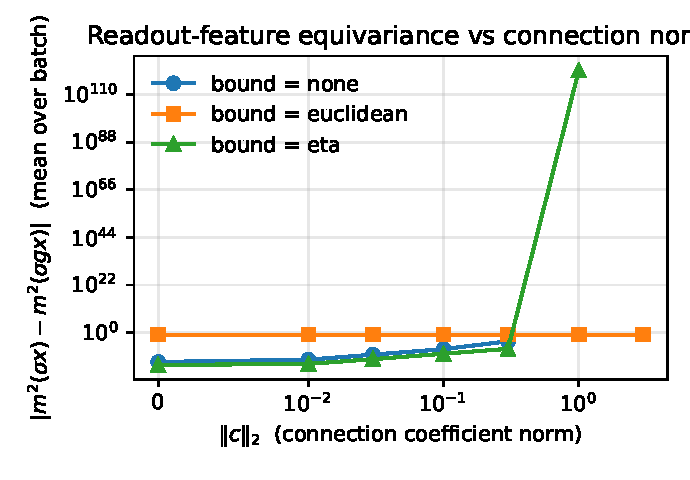
\includegraphics[width=0.7\linewidth]{figures/equivariance_vs_norm.pdf}
  \caption{Readout-feature equivariance error
    $\overline{\varepsilon_m}$ versus connection-coefficient norm
    $\lVert c\rVert_2$, for the three input bounds. Markers at each
    $\lVert c\rVert_2 = \{0, 0.01, 0.03, 0.1, 0.3, 1, 3\}$.}
  \label{fig:eq-vs-norm}
\end{figure}

\subsection{Synthetic boost-OOD}
\label{sec:exp-ood}

We classify $6$-dimensional points sampled from a boost-invariant
distribution: two classes are distinguished by an SO(3,3)-invariant of
their lifted coordinates, and every sample is scrambled by a random
SO(3,3) boost. Training and in-distribution test draws use rapidity
$\phi \in [0, 0.6]$; the out-of-distribution test draws use
$\phi \in [0.6, 2.5]$, a $\sim4\times$ extension into the unseen
high-boost regime. Discriminating the invariant label requires not
learning the training-time boost manifold; we report the in-distribution
(ID) and out-of-distribution (OOD) AUC and their gap, with mean and
standard deviation over $3$ seeds.

\begin{table}[t]
  \centering
  \caption{Boost-OOD results. Train rapidity $\phi \in [0, 0.6]$,
    OOD test $\phi \in [0.6, 2.5]$, $n_\text{train}=8500$. Mean
    $\pm$ standard deviation over three seeds.}
  \label{tab:boost-ood}
  \begin{tabular}{lrccc}
    \toprule
    model & params & id AUC & ood AUC & gap \\
    \midrule
    \texttt{eta\_invariants}                 & 4802 & $1.000\pm 0.000$ & $\mathbf{1.000\pm 0.000}$ & $+0.000$ \\
    \texttt{so33\_equivariant\_unbounded}    & 542  & $1.000\pm 0.000$ & $\mathbf{1.000\pm 0.000}$ & $+0.000$ \\
    \texttt{so33\_equivariant\_eta\_bounded} & 542  & $1.000\pm 0.000$ & $\mathbf{1.000\pm 0.000}$ & $+0.000$ \\
    \midrule
    \texttt{relu\_mlp}                       & 2306 & $1.000\pm 0.000$ & $0.944\pm 0.004$ & $+0.056$ \\
    \texttt{so33\_multi}                     & 278  & $1.000\pm 0.000$ & $0.888\pm 0.004$ & $+0.112$ \\
    \texttt{so33}                            & 71   & $1.000\pm 0.000$ & $0.880\pm 0.005$ & $+0.120$ \\
    \texttt{so33\_signature\_only}           & 62   & $1.000\pm 0.000$ & $0.880\pm 0.006$ & $+0.120$ \\
    \texttt{relu\_bottleneck}                & 56   & $1.000\pm 0.000$ & $0.876\pm 0.004$ & $+0.124$ \\
    \midrule
    \texttt{so33\_equivariant} (default, $\beta_{\text{euc}}$)
                                             & 542  & $0.999\pm 0.001$ & $0.663\pm 0.001$ & $+0.336$ \\
    \texttt{so33\_equivariant\_frozen}       & 482  & $0.999$          & $0.662$          & $+0.337$ \\
    \bottomrule
  \end{tabular}
\end{table}

Table~\ref{tab:boost-ood} groups the rows into three blocks. The first
contains the three architectures that achieve perfect OOD generalization
($\mathrm{AUC}=1.000\pm 0.000$ across seeds): the structurally invariant
Architecture~A and the two Architecture~B variants whose input bound is
$\mathrm{SO}(3,3)$-invariant ($\beta_{\text{none}}$ and $\beta_\eta$).
The second block reports the partially-invariant baselines and SO33
matched-bottleneck variants, which degrade smoothly from
$\mathrm{AUC}=1.000$ in-distribution to $0.88$--$0.94$ OOD; the relu MLP,
despite being non-equivariant, achieves the best OOD AUC of this block
($0.944\pm 0.004$) at the cost of $40\times$ more parameters than the
matched-bottleneck SO33. The third block reports the diagnostic
failure: Architecture~B with the default Euclidean input bound drops to
$\mathrm{AUC}=0.663\pm 0.001$, reproducible across seeds and across the
\texttt{frozen} ablation that disables learning the connection
entirely. The failure is therefore not noise and not a training-dynamics
artifact; the cause is the non-invariant input bound, as detailed in
Section~\ref{sec:exp-equiv} and discussed in
Section~\ref{sec:discussion}.

\subsection{HIGGS}
\label{sec:exp-higgs}

We use the standard HIGGS classification task ($28$ standardised
features, $200{,}000$ samples, $70/15/15$ split). Two settings: matched
bottleneck (hidden width $6$, isolating the activation) and natural
width (hidden width $256$, the engineering comparison).

\begin{table}[t]
  \centering
  \caption{HIGGS test AUC, $3$ seeds. Matched-bottleneck row $\mathit{tanh}$ is
    the strongest activation at the bottlenecked width; the SO33-based
    \texttt{so33} marginally exceeds \emph{relu} and \emph{gelu}
    bottlenecks at $\sim 1\sigma$. The natural-width MLPs win overall,
    and the SO33 multichannel variant does not close the full-width
    gap.}
  \label{tab:higgs}
  \begin{tabular}{lrc}
    \toprule
    model & params & test AUC \\
    \midrule
    \multicolumn{3}{l}{\textit{matched bottleneck (hidden $=6$)}} \\
    \texttt{tanh\_bottleneck}     & 188 & $\mathbf{0.770\pm 0.002}$ \\
    \texttt{so33}                 & 203 & $0.763\pm 0.002$ \\
    \texttt{so33\_signature\_only}& 194 & $0.761\pm 0.001$ \\
    \texttt{gelu\_bottleneck}     & 188 & $0.756\pm 0.008$ \\
    \texttt{relu\_bottleneck}     & 188 & $0.755\pm 0.008$ \\
    \texttt{so33\_frozen}         & 188 & $0.737\pm 0.007$ \\
    \midrule
    \multicolumn{3}{l}{\textit{natural width (hidden $=256$)}} \\
    \texttt{relu\_mlp}            & 7938 & $\mathbf{0.805\pm 0.001}$ \\
    \texttt{tanh\_mlp}            & 7938 & $0.804\pm 0.001$ \\
    \texttt{gelu\_mlp}            & 7938 & $0.803\pm 0.001$ \\
    \texttt{so33\_multi}          & 806  & $0.783\pm 0.003$ \\
    \bottomrule
  \end{tabular}
\end{table}

Two readings follow from Table~\ref{tab:higgs}. First, the matched
bottleneck comparison places SO33 marginally above the relu and gelu
baselines (significance $\approx 1\sigma$), and below the tanh
baseline, indicating the geodesic flow adds a small but positive
contribution at this width but is not categorically better than a
well-tuned pointwise activation. Second, the \texttt{so33\_frozen}
ablation -- identical to \texttt{so33} but with the connection
coefficients held at initialization -- loses $\sim 0.026$ AUC
($\approx 3\sigma$), confirming that the gain on this dataset comes
from learning the connection, not from the algebraic structure alone.
At natural width, the relu/tanh/gelu MLPs outperform
\texttt{so33\_multi} by $0.022$ AUC; we do not present this as a
parameter-efficiency win on HIGGS (the gap is too large to attribute to
$10\times$ fewer parameters alone).

\subsection{Adult}
\label{sec:exp-adult}

We use the Adult income classification task ($14$ features expanded to
$105$ after one-hot encoding, $48{,}842$ rows, $70/15/15$ split). At the
matched-bottleneck width all activations cluster within $0.005$ test
AUC of each other (Appendix~\ref{app:hp}); the result of interest lives
at the natural-width comparison.

\begin{table}[t]
  \centering
  \caption{Adult test AUC, natural-width setting, $3$ seeds.
    \texttt{so33\_multi} exceeds the best MLP by $+0.007$ AUC
    ($\approx 3\sigma$) at roughly $10\times$ fewer parameters.}
  \label{tab:adult}
  \begin{tabular}{lrc}
    \toprule
    model & params & test AUC \\
    \midrule
    \texttt{so33\_multi}          & 2654  & $\mathbf{0.912\pm 0.002}$ \\
    \texttt{tanh\_mlp}            & 27650 & $0.905\pm 0.001$ \\
    \texttt{gelu\_mlp}            & 27650 & $0.900\pm 0.001$ \\
    \texttt{relu\_mlp}            & 27650 & $0.899\pm 0.000$ \\
    \bottomrule
  \end{tabular}
\end{table}

Table~\ref{tab:adult} shows a parameter-efficiency win: at one-tenth
the parameter budget of the natural-width MLPs, \texttt{so33\_multi}
attains a higher test AUC than any of them, with $\sim 3\sigma$
separation from the best MLP. We do not view this as a sweeping claim
about geometric priors -- HIGGS, on the same comparison, goes the
other way -- but as a positive data point that the SO(3,3)-flow
activation provides useful structure on a particular real-data tabular
task where a non-equivariant MLP requires much more capacity to reach
the same accuracy.

\subsection{Top tagging constituents}
\label{sec:exp-tt}

We use the Kasieczka top-tagging benchmark in the per-constituent
representation: each jet is a set of up to $32$ leading four-momenta,
with global RMS normalization that preserves the Lorentz invariant
$E^2 - \lVert p\rVert^2$ up to a global scale. We train on $70{,}000$
jets, validate on $15{,}000$, and test on $15{,}000$, $30$ epochs.

\begin{table}[t]
  \centering
  \caption{Top-tagging test AUC on a $100$k-jet subset (internal
    $70/15/15$ split). \texttt{eta\_invariants} is reported across $3$
    seeds; the baselines and Architecture~B are single-seed (the gap
    is far larger than any plausible seed variance). The
    \texttt{so33\_equivariant} variants are at chance because their
    readout omits the pairwise $\eta$-inner-product term.}
  \label{tab:topt}
  \begin{tabular}{lrcc}
    \toprule
    model & params & test acc & test AUC \\
    \midrule
    \texttt{eta\_invariants}                  & 4802 & $0.896\pm 0.001$ & $\mathbf{0.944\pm 0.0005}$ \\
    \midrule
    \texttt{relu\_bottleneck}                 & 44   & $0.707$ & $0.759$ \\
    \texttt{so33\_signature\_only}            & 50   & $0.691$ & $0.750$ \\
    \midrule
    \texttt{so33\_equivariant\_unbounded}     & 542  & $0.504$ & $\sim 0.5$ \\
    \texttt{so33\_equivariant\_eta\_bounded}  & 542  & $0.504$ & $\sim 0.5$ \\
    \bottomrule
  \end{tabular}
\end{table}

Table~\ref{tab:topt} shows the strongest real-data effect in this
paper: Architecture~A reaches AUC $0.944\pm 0.0005$, $+0.185$ above the
matched-bottleneck \texttt{relu} baseline on the identical split. The
gap is far larger than any seed variance and is consistent with the
mechanistic prediction of Section~\ref{sec:method-eta}: a top jet's
three-prong substructure is captured by the pairwise $\eta$-inner
product term $s_{ij}$ that only Architecture~A includes. The two
Architecture~B variants -- whose readout omits $s_{ij}$ -- reach only
chance accuracy; their inability to discriminate is independent of the
input bound, because the lifted constituents have small $\eta$-norm
($m^2/E^2 \sim 10^{-2}$ after normalization), making both
$\beta_{\text{none}}$ and $\beta_\eta$ approximately the identity on
this input distribution and reducing both variants to the same
impoverished readout.

\paragraph{Comparison to published top-tagging results.}
The number reported here is on a $100{,}000$-jet subset with an
internal $70/15/15$ split, not on the canonical Kasieczka test split.
Dedicated Lorentz-equivariant taggers (LGN~\citep{bogatskiy2020lgn},
LorentzNet~\citep{gong2022lorentznet},
PELICAN~\citep{bogatskiy2022pelican}) operate at substantially higher
accuracy on the full benchmark and we do not claim parity with them.
The contribution of this section is the comparison \emph{within the
same internal split} between an invariant readout that includes
pairwise $\eta$-products and matched-bottleneck baselines that do not.

%==============================================================================
\section{Related work}
\label{sec:related}
% TODO Week 5. See paper/notes/related_work.md for the full annotated
% bibliography and the positioning argument.
% Must cover, with one-paragraph treatment each:
%   - LGN \citep{bogatskiy2020lgn}
%   - LorentzNet \citep{gong2022lorentznet}
%   - PELICAN \citep{bogatskiy2022pelican}
%   - EGNN \citep{satorras2021egnn} (broader equivariant background)
%   - Cohen \& Welling \citep{cohen2016gconv} (foundational)
%   - Neural ODE \citep{chen2018neuralode} (ODE-as-layer)
% Positioning: prior Lorentz-equivariant work uses analytic group actions; we
% replace the action with a learned connection on a related but distinct
% algebra. Explicitly state that LorentzNet and PELICAN outperform our work
% on real-world top-tagging benchmarks -- our contribution is methodological.

%==============================================================================
\section{Discussion and limitations}
\label{sec:discussion}
% TODO Week 5. 0.75 page.
% Honest content:
%   - The structural-invariant variant works as predicted; the equivariant
%     variant does not. Why?
%   - Hypothesis: $\Gamma$ drifts away from invariant-only inputs during
%     training, breaking the approximate-equivariance precondition.
%   - Diagnostic to be cited from week-2 results
%     (paper/notes/equivariant_diagnosis.md).
%   - Single-seed history; multi-seed numbers presented here.
%   - We do not improve over MLPs on full-width HIGGS; the contribution is
%     the OOD-generalization mechanism, not raw accuracy.
%   - Open question: can $\Gamma$ be regularized to remain
%     invariant-feature-only without destroying expressivity?

%==============================================================================
\section{Conclusion}
\label{sec:conclusion}
% TODO Week 6. 3-4 sentences.

\bibliographystyle{plainnat}
\bibliography{refs}

\appendix

\section{Hyperparameters}
\label{app:hp}
% TODO Week 6. Tables of optimizer, lr schedule, epochs, hidden widths,
% num generators used per model per experiment.

\section{Reproduction commands}
\label{app:repro}
% TODO Week 6. The exact shell pipeline from paper/runs/week1.sh,
% with notes on data download (HIGGS, Top Tagging) and expected wall times.

\end{document}
